% Options for packages loaded elsewhere
\PassOptionsToPackage{unicode}{hyperref}
\PassOptionsToPackage{hyphens}{url}
%
\documentclass[
]{article}
\usepackage{amsmath,amssymb}
\usepackage{lmodern}
\usepackage{iftex}
\ifPDFTeX
  \usepackage[T1]{fontenc}
  \usepackage[utf8]{inputenc}
  \usepackage{textcomp} % provide euro and other symbols
\else % if luatex or xetex
  \usepackage{unicode-math}
  \defaultfontfeatures{Scale=MatchLowercase}
  \defaultfontfeatures[\rmfamily]{Ligatures=TeX,Scale=1}
\fi
% Use upquote if available, for straight quotes in verbatim environments
\IfFileExists{upquote.sty}{\usepackage{upquote}}{}
\IfFileExists{microtype.sty}{% use microtype if available
  \usepackage[]{microtype}
  \UseMicrotypeSet[protrusion]{basicmath} % disable protrusion for tt fonts
}{}
\makeatletter
\@ifundefined{KOMAClassName}{% if non-KOMA class
  \IfFileExists{parskip.sty}{%
    \usepackage{parskip}
  }{% else
    \setlength{\parindent}{0pt}
    \setlength{\parskip}{6pt plus 2pt minus 1pt}}
}{% if KOMA class
  \KOMAoptions{parskip=half}}
\makeatother
\usepackage{xcolor}
\IfFileExists{xurl.sty}{\usepackage{xurl}}{} % add URL line breaks if available
\IfFileExists{bookmark.sty}{\usepackage{bookmark}}{\usepackage{hyperref}}
\hypersetup{
  hidelinks,
  pdfcreator={LaTeX via pandoc}}
\urlstyle{same} % disable monospaced font for URLs
\usepackage{longtable,booktabs,array}
\usepackage{calc} % for calculating minipage widths
% Correct order of tables after \paragraph or \subparagraph
\usepackage{etoolbox}
\makeatletter
\patchcmd\longtable{\par}{\if@noskipsec\mbox{}\fi\par}{}{}
\makeatother
% Allow footnotes in longtable head/foot
\IfFileExists{footnotehyper.sty}{\usepackage{footnotehyper}}{\usepackage{footnote}}
\makesavenoteenv{longtable}
\usepackage{graphicx}
\makeatletter
\def\maxwidth{\ifdim\Gin@nat@width>\linewidth\linewidth\else\Gin@nat@width\fi}
\def\maxheight{\ifdim\Gin@nat@height>\textheight\textheight\else\Gin@nat@height\fi}
\makeatother
% Scale images if necessary, so that they will not overflow the page
% margins by default, and it is still possible to overwrite the defaults
% using explicit options in \includegraphics[width, height, ...]{}
\setkeys{Gin}{width=\maxwidth,height=\maxheight,keepaspectratio}
% Set default figure placement to htbp
\makeatletter
\def\fps@figure{htbp}
\makeatother
\setlength{\emergencystretch}{3em} % prevent overfull lines
\providecommand{\tightlist}{%
  \setlength{\itemsep}{0pt}\setlength{\parskip}{0pt}}
\setcounter{secnumdepth}{-\maxdimen} % remove section numbering
\ifLuaTeX
  \usepackage{selnolig}  % disable illegal ligatures
\fi

\author{}
\date{}

\begin{document}

\textbf{MULTI-DISEASE DETECTION IN RETINAL IMAGING}

\textbf{BASED ON ENSEMBLING HETEROGENEOUS DEEP LEARNING MODELS}

\emph{Dominik Müller1, Iñaki Soto-Rey1,2 and Frank Kramer1}

1 IT-Infrastructure for Translational Medical Research, University of
Augsburg, Germany

2 Medical Data Integration Center, University Hospital Augsburg, Germany

\textbf{ABSTRACT}

Preventable or undiagnosed visual impairment and blindness affect
billion of people worldwide. Automated multi-disease detection models
offer great potential to address this problem via clinical decision
support in diagnosis. In this work, we proposed an innovative
multi-disease detection pipeline for retinal imaging which utilizes
ensemble learning to combine the predictive capabilities of several
heterogeneous deep convolutional neural network models. Our pipeline
includes state-of-the-art strategies like transfer learning, class
weighting, real-time image augmentation and Focal loss utilization.
Furthermore, we integrated ensemble learning techniques like
heterogeneous deep learning models, bagging via 5-fold cross-validation
and stacked logistic regression models. Through internal and external
evaluation, we were able to validate and demonstrate high accuracy and
reliability of our pipeline, as well as the comparability with other
stateof-the-art pipelines for retinal disease prediction.

\begin{quote}
\emph{\textbf{Index Terms---}} Retinal Disease Detection, Ensemble
Learning, Class
\end{quote}

Imbalance, Multi-label Image Classification, Deep Learning

\textbf{1. INTRODUCTION}

Even if the medical progress in the last 30 years made it possible to
successfully treat the majority of diseases causing visual impairment,
growing and aging populations lead to an increasing challenge in retinal
disease diagnosis {[}1{]}. The World Health Organization (WHO) estimates
the prevalence of blindness and visual impairment to 2.2 billion people
worldwide, of whom at least 1 billion affections could have been
prevented or is yet to be addressed {[}2{]}. Early detection and correct
diagnosis are essential to forestall disease course and prevent
blindness.

The use of clinical decision support (CDS) systems for diagnosis has
been increasing over the past decade {[}3{]}. Recently, modern deep
learning models allow automated and reliable classification of medical
images with remarkable accuracy comparable to physicians {[}4{]}.
Nevertheless, these models often lack capabilities to detect rare
pathologies such as central retinal artery occlusion or anterior
ischemic optic neuropathy {[}5{]}, {[}6{]}.

\begin{quote}
In this study we push towards creating a highly accurate and reliable
multi-disease detection pipeline based on ensemble, transfer and deep
learning techniques. Furthermore, we utilize the new Retinal Fundus
Multi-Disease Image Dataset (RFMiD) containing various rare and
challenging conditions to demonstrate our detection capabilities for
uncommon diseases.
\end{quote}

\textbf{2. METHODS}

\begin{quote}
The implemented medical image classification pipeline can be summarized
in the following core steps and is illustrated in Fig. 1:\\
- Stratified multi-label 5-fold cross-validation\\
- Class weighted Focal loss and up-sampling\\
- Extensive real-time image augmentation\\
- Multiple deep learning model architectures\\
- Ensemble learning strategies: bagging and stacking\\
- Individual training for multi-disease labels and disease risk
detection utilizing transfer learning on ImageNet\\
- Stacked binary logistic regression models for distinct
classification\\
\textbf{2.1. Retinal Imaging Dataset}\\
The RFMiD dataset consists of 3200 retinal images for which 1920 images
were used as training dataset {[}7{]}. The fundus images were captured
by three different fundus cameras having a resolution of 4288x2848 (277
images), 2048x1536 (150 images) and 2144x1424 (1493 images),
respectively.

\textbf{Tab. 1.} Annotation frequency for each class in the dataset.
\end{quote}

\begin{longtable}[]{@{}
  >{\raggedright\arraybackslash}p{(\columnwidth - 4\tabcolsep) * \real{0.33}}
  >{\raggedright\arraybackslash}p{(\columnwidth - 4\tabcolsep) * \real{0.33}}
  >{\raggedright\arraybackslash}p{(\columnwidth - 4\tabcolsep) * \real{0.33}}@{}}
\toprule
\begin{minipage}[b]{\linewidth}\raggedright
\begin{quote}
\textbf{Disease} \textbf{Samples}
\end{quote}
\end{minipage} & \begin{minipage}[b]{\linewidth}\raggedright
\begin{quote}
\textbf{Disease} \textbf{Samples}
\end{quote}
\end{minipage} & \begin{minipage}[b]{\linewidth}\raggedright
\begin{quote}
\textbf{Disease} \textbf{Samples}
\end{quote}
\end{minipage} \\
\midrule
\endhead
\begin{minipage}[t]{\linewidth}\raggedright
\begin{longtable}[]{@{}
  >{\raggedright\arraybackslash}p{(\columnwidth - 2\tabcolsep) * \real{0.50}}
  >{\raggedright\arraybackslash}p{(\columnwidth - 2\tabcolsep) * \real{0.50}}@{}}
\toprule
\begin{minipage}[b]{\linewidth}\raggedright
\begin{quote}
D. Risk
\end{quote}
\end{minipage} & 1519 \\
\midrule
\endhead
MH & 317 \\
\begin{minipage}[t]{\linewidth}\raggedright
\begin{quote}
BRVO
\end{quote}
\end{minipage} & 73 \\
LS & 47 \\
\begin{minipage}[t]{\linewidth}\raggedright
\begin{quote}
ODC
\end{quote}
\end{minipage} & 282 \\
AH & 16 \\
\begin{minipage}[t]{\linewidth}\raggedright
\begin{quote}
AION
\end{quote}
\end{minipage} & 17 \\
RS & 43 \\
\begin{minipage}[t]{\linewidth}\raggedright
\begin{quote}
RPEC
\end{quote}
\end{minipage} & 22 \\
\begin{minipage}[t]{\linewidth}\raggedright
\begin{quote}
OTHER
\end{quote}
\end{minipage} & 34 \\
\bottomrule
\end{longtable}
\end{minipage} & \begin{minipage}[t]{\linewidth}\raggedright
\begin{longtable}[]{@{}
  >{\raggedright\arraybackslash}p{(\columnwidth - 2\tabcolsep) * \real{0.50}}
  >{\raggedright\arraybackslash}p{(\columnwidth - 2\tabcolsep) * \real{0.50}}@{}}
\toprule
\begin{minipage}[b]{\linewidth}\raggedright
\begin{quote}
DR
\end{quote}
\end{minipage} & 376 \\
\midrule
\endhead
\begin{minipage}[t]{\linewidth}\raggedright
\begin{quote}
DN
\end{quote}
\end{minipage} & 138 \\
\begin{minipage}[t]{\linewidth}\raggedright
\begin{quote}
TSLN
\end{quote}
\end{minipage} & 186 \\
\begin{minipage}[t]{\linewidth}\raggedright
\begin{quote}
MS
\end{quote}
\end{minipage} & 15 \\
\begin{minipage}[t]{\linewidth}\raggedright
\begin{quote}
CRVO
\end{quote}
\end{minipage} & 28 \\
\begin{minipage}[t]{\linewidth}\raggedright
\begin{quote}
ODP
\end{quote}
\end{minipage} & 65 \\
PT & 11 \\
\begin{minipage}[t]{\linewidth}\raggedright
\begin{quote}
CRS
\end{quote}
\end{minipage} & 32 \\
\begin{minipage}[t]{\linewidth}\raggedright
\begin{quote}
MHL
\end{quote}
\end{minipage} & 11 \\
\bottomrule
\end{longtable}
\end{minipage} & \begin{minipage}[t]{\linewidth}\raggedright
\begin{longtable}[]{@{}
  >{\raggedright\arraybackslash}p{(\columnwidth - 2\tabcolsep) * \real{0.50}}
  >{\raggedright\arraybackslash}p{(\columnwidth - 2\tabcolsep) * \real{0.50}}@{}}
\toprule
\begin{minipage}[b]{\linewidth}\raggedright
\begin{quote}
ARMD
\end{quote}
\end{minipage} & 100 \\
\midrule
\endhead
\begin{minipage}[t]{\linewidth}\raggedright
\begin{quote}
MYA
\end{quote}
\end{minipage} & 101 \\
\begin{minipage}[t]{\linewidth}\raggedright
\begin{quote}
ERM
\end{quote}
\end{minipage} & 14 \\
\begin{minipage}[t]{\linewidth}\raggedright
\begin{quote}
CSR
\end{quote}
\end{minipage} & 37 \\
TV & 6 \\
ST & 5 \\
RT & 14 \\
\begin{minipage}[t]{\linewidth}\raggedright
\begin{quote}
EDN
\end{quote}
\end{minipage} & 15 \\
RP & 6 \\
\bottomrule
\end{longtable}
\end{minipage} \\
\bottomrule
\end{longtable}

\begin{quote}
Preprint - March 2021 Page 1 / 6

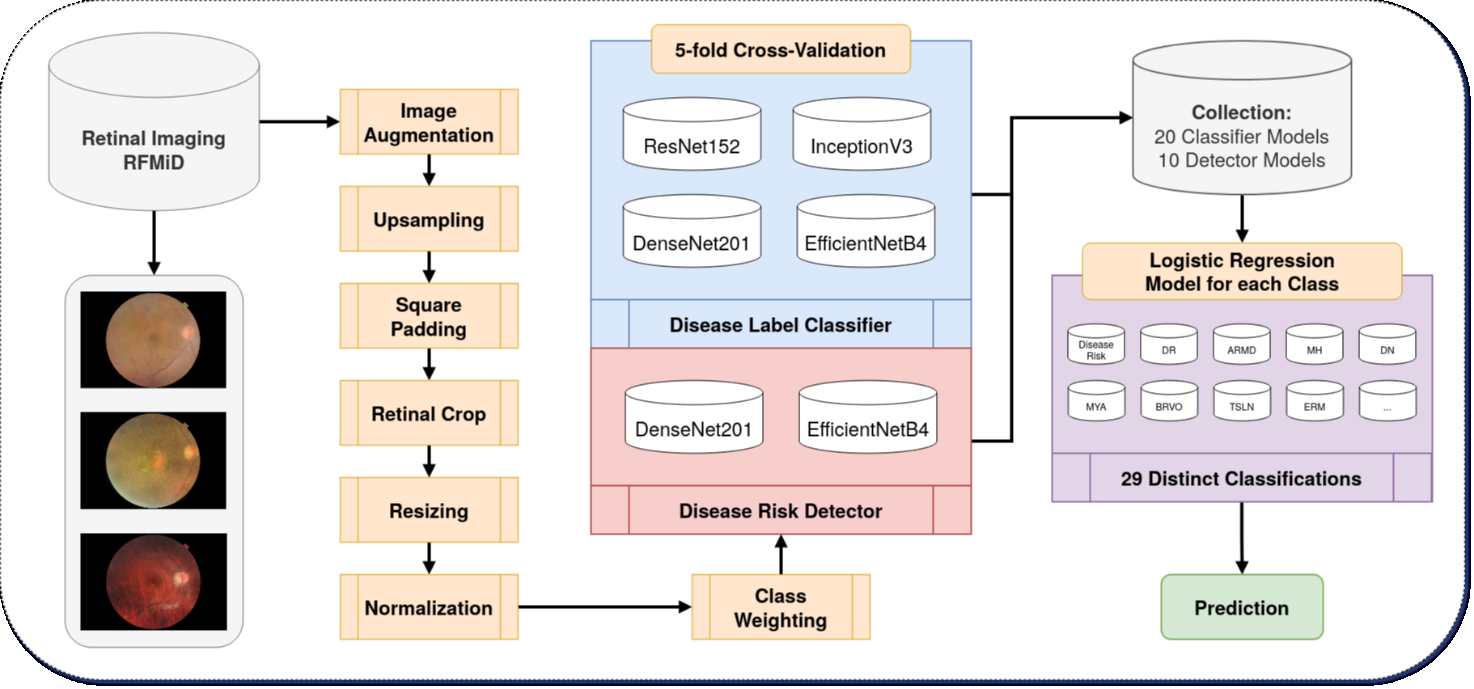
\includegraphics[width=6.70417in,height=3.13333in]{vertopal_2f1cfafaf78f44c9b64931ec8d4445e5/media/image1.png}

\textbf{Fig. 1}. Flowchart diagram of the implemented medical image
analysis pipeline for multi-disease detection in retinal imaging. The
workflow is starting with the retinal imaging dataset (RFMiD) and ends
with computed predictions for novel images.
\end{quote}

The images were annotated with 46 conditions, including various rare and
challenging diseases, through adjudicated consensus of two senior
retinal experts. These 46 conditions are represented by the following
classes, which are also listed in Tab. 1: An overall normal/abnormal
class, 27 specific condition classes and 1 `OTHER' class consisting of
the remaining extremely rare conditions. Besides the training dataset,
the organizers of the RIADD challenge hold 1280 images back for external
validation and testing datasets to ensure robust evaluation {[}7{]},
{[}8{]}.

\textbf{2.2. Preprocessing and Image Augmentation}\\
In order to simplify the pattern finding process of the deep learning
model, as well as to increase data variability, we applied several
preprocessing methods.

\begin{quote}
We utilized extensive image augmentation for up-
\end{quote}

sampling to balance class distribution and real-time augmentation during
training to obtain novel and unique images in each epoch. The
augmentation techniques consisted of rotation, flipping, and altering in
brightness, saturation, contrast and hue. Through the up-sampling, it
was ensured that each label occurred at least 100 times in the dataset
which increased the total number of training images from 1920 to 3354.

Afterwards, all images were square padded in order to avoid aspect ratio
loss during posterior resizing. The retinal images were also cropped to
ensure that the fundus is center located in the image. The cropping was
performed individually for each microscope resolution and resulted in
the following image shapes: 1424x1424, 1536x1536 and 3464x3464 pixels.
The images were then resized to model

\begin{quote}
input sizes according to the neural network architecture, which was
380x380 for EfficientNetB4, 299x299 for InceptionV3 and 244x244 for all
remaining architectures {[}9{]}--{[}12{]}.

Before feeding the image to the deep convolutional neural network, we
applied value intensity normalization as last preprocessing step. The
intensities were zero-centered via the Z-Score normalization approach
based on the mean and standard deviation computed on the ImageNet
dataset {[}13{]}.

\textbf{2.3. Deep Learning Models}\\
The state-of-the-art for medical image classification are the unmatched
deep convolutional neural network models {[}4{]}, {[}14{]}.
Nevertheless, the hyper parameter configuration and architecture
selection are highly dependent on the required computer vision task, as
well as the key difference between pipelines {[}4{]}, {[}15{]}. Thus,
our pipeline combines two different types of image classification
models: The disease risk detector for binary classifying normal/abnormal
images and the disease label classifier for multi-label annotation of
abnormal images.

Both model types were pretrained on the ImageNet

dataset {[}13{]}. For the fitting process, we applied a transfer
learning training, with frozen architecture layers except for the
classification head, and a fine-tuning strategy with unfrozen layers.
Whereas the transfer learning fitting was performed for 10 epochs using
the Adam optimization with an initial learning rate of 1-E04, the
fine-tuning had a maximal training time of 290 epochs and using a
dynamic learning rate for the Adam optimization starting from 1-E05 to a
maximum decrease to 1-E07 (decreasing factor of 0.1

Preprint - March 2021 Page 2 / 6
\end{quote}

after 8 epochs without improvement on the monitored validation loss)
{[}16{]}. Furthermore, an early stopping and model checkpoint technique
was utilized for the fine-tuning process, stopping after 20 epochs
without improvement (after epoch 60) and saving the best model measured
according to the validation loss. Instead of defining an epoch as a
cycle through the full training dataset, we establish an epoch to have
250 iterations. This allowed to increase the number of seen batches and,
thus, to increase the information given to the model during the fitting
process of an epoch. As training loss function, we utilized the weighted
Focal loss from \emph{Lin et al.} {[}17{]}.

\begin{quote}
FL(𝑝𝑡) = −𝛼𝑡(1 − 𝑝𝑡)𝛾 log (𝑝𝑡) (1)
\end{quote}

In the above formula, \emph{pt} is the probability for the correct
ground truth class \emph{t}, \emph{γ} a tunable focusing parameter
(which we set to 2.0) and \emph{αt} the associated weight for class
\emph{t}.

\emph{2.3.1 Disease Risk Detector}\\
The disease risk detector was established as a binary classifier of the
disease risk class for general categorizing between normal and abnormal
retinal images. Thus, this model type was trained using only the disease
risk class and ignoring all multi-label annotations. Rather than using a
single model architecture, we trained multiple models based on the
DenseNet201 and EfficientNetB4 architecture {[}9{]}, {[}10{]}. For class
weight computation, we divided the number of samples by the
multiplication of the number of classes (2 for a binary classification)
with the number of class occurrences in the dataset.

\emph{2.3.2 Disease Label Classifier}\\
In contrast, the disease label classifier was established as multi-label
classifier of all 28 remaining classes (excluding disease risk) and was
trained on the one hot encoded array of the disease labels. Furthermore,
we utilized four different architectures for this model type: ResNet152,
InceptionV3, DenseNet201 and EfficientNetB4 {[}9{]}--{[}12{]}. Identical
to class weight computation of the disease risk detector, we computed
the weights individually as binary classification for each class. Even
if this classifier is provided with all classes, the binary weights
balance the decision for each label individually.

\textbf{2.4. Ensemble Learning Strategy}\\
\emph{2.4.1 Bagging}\\
Next to the utilization of multiple architecture, we also applied a
5-fold cross-validation based as a bagging approach for ensemble
learning. Our aim was to create a large variety of models which were
trained on different subsets of the training data. This approach not
only allowed a more efficient usage of the available training data, but
also increased the

\begin{quote}
reliability of a prediction. This strategy resulted in an ensemble of 10
disease risk detector models (2 architectures with each 5 folds) and 20
disease label classifier models (4 architectures with each 5 folds).

\emph{2.4.2 Stacking}\\
For combining the predictions of our, in total, 30 models, we integrated
a stacking setup. On top of all deep convolutional neural networks, we
applied a binary logistic regression algorithm for each class,
individually. Thus, the predictions of all models were utilized as input
for computing the classification of a single class. This approach
allowed combining the information of all other class predictions to
derive an inference for one single class. Overall, this strategy
resulted in 29 distinct logistic regression models (1 for disease risk
and 28 for each disease-label including the `other' class). The
individual predicted class probabilities are then concatenated to the
final prediction.

The logistic regression models were also trained with the same 5-fold
cross-validation sampling on a heavily augmented version of the training
dataset to avoid overfitting as well as avoiding training the logistic
regression models on already seen images from the neural network models.
As logistic regression solver, we utilized the large-scale
boundconstrained optimization (short: `LBFGS') from \emph{Zhu et al}.
{[}18{]}.

\textbf{3. RESULTS AND DISCUSSION}

The sequential training of a complete cross-validation for one
architecture on a single NVIDIA TITAN RTX GPU took around 13.5 hours
with 63 epochs on average for each deep convolutional neural network
model. Logistic Regression training required less than 30 minutes for
all class models combined. No signs of overfitting were observed for the
disease label classifiers through validation monitoring, as it can be
seen in Fig. 2. However, the disease risk detectors showed a strong
trend to overfit after the transfer learning phase. Through our strategy
to use the model with the best

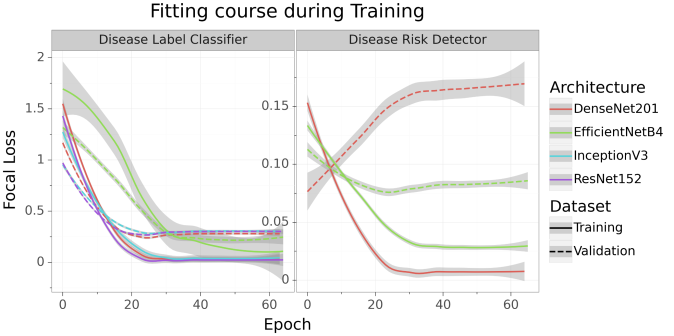
\includegraphics[width=3.375in,height=1.68472in]{vertopal_2f1cfafaf78f44c9b64931ec8d4445e5/media/image2.png}\textbf{Fig.
2.} Loss course during the training process for training and validation
data. The lines were computed via locally estimated scatterplot
smoothing and represent the average loss across all folds. The gray
areas around the lines represent the confidence intervals.

Preprint - March 2021 Page 3 / 6

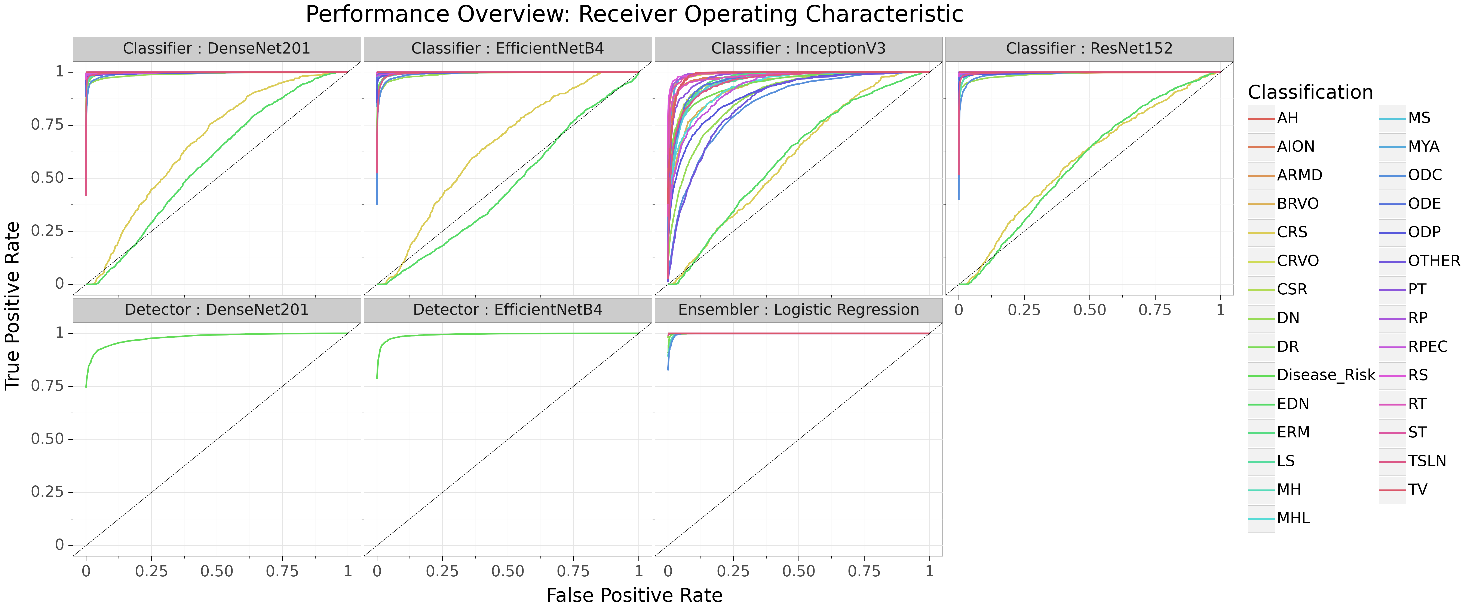
\includegraphics[width=6.70417in,height=2.76944in]{vertopal_2f1cfafaf78f44c9b64931ec8d4445e5/media/image3.png}
\end{quote}

\textbf{Fig. 3.} Receiver operating characteristic (ROC) curves for each
model type applied in our pipeline. The ROC curves showing the
individual model performance measured by the true positive and false
positive rate. The cross-validation models were macro-averaged for each
model type to reduce illustration complexity.

validation loss, it was still possible to obtain a powerful model for
detection.

\textbf{3.1. Internal Performance Evaluation}\\
For estimating the performance of our pipeline, we utilized the
validation subsets of the 5-fold cross-validation models from the
heavily augmented version of our dataset. This approach allowed to
obtain testing samples which were never seen in the training process for
reliable performance evaluation. For the complex multi-label evaluation,
we computed the popular area under the receiver operating characteristic
(AUROC) curve, as well as the mean average precision (mAP). Both scores
were macro-averaged over classes and cross-validation folds to reduce
complexity.

Our multi-disease detection pipeline revealed a strong and robust
classification performance with the capability to also detect rare
conditions accurately in retinal images. Whereas the disease label
classifier models separately only achieved an AUROC of around 0.97 and a
mAP of 0.93, the disease risk detectors demonstrated to have a really
strong predictive power of 0.98 up to 0.99 AUROC and mAP. However, for
the classifiers the InceptionV3 architecture indicated to have the worst
performance compared to the other architectures with only 0.93 AUROC and
0.66 mAP. The associated receiver operating characteristics of the
models are illustrated in Fig. 3.

Training a strong multi-label classifier is in general a complex task,
however, the extreme class imbalance between the conditions revealed a
hard challenge for building a reliable model {[}19{]}, {[}20{]}. Our
applied up-sampling and class weighting technique demonstrated to have a
critical boost on the predictive capabilities of the classifier models.
Nearly all labels were able to be accurately detected,

\begin{quote}
including the `OTHER' class consisting of various extremely rare
conditions. Nevertheless, the two classes `EDN' and `CRS' were the most
challenging conditions for all classifier models. Both classes belong to
very rare conditions, combined with less than 1.2\% occurrence in the
original and 2.5\% occurrence in the up-sampled dataset. Still, our
stacked logistic regression algorithm was able to balance this issue and
infer the correct `EDN' and `CRS' classifications through context.
Overall, our applied ensemble learning strategies resulted in a
significant performance improvement compared to the individual deep
convolutional neural network models. More details on the internal
performance evaluation are listed in Tab. 2.

\textbf{3.2. External Evaluation through the RIADD Challenge}
Furthermore, we participated at the RIADD challenge which was organized
by the authors of the RFMiD dataset {[}7{]}, {[}8{]}. The challenge
participation allowed not only an independent

\textbf{Tab. 2}. Achieved results of the internal performance evaluation
showing the average AUROC and mAP score for each model utilized in our
pipeline. The scores were macroaveraged across all cross-validation
folds and classes.
\end{quote}

\begin{longtable}[]{@{}
  >{\raggedright\arraybackslash}p{(\columnwidth - 2\tabcolsep) * \real{0.50}}
  >{\raggedright\arraybackslash}p{(\columnwidth - 2\tabcolsep) * \real{0.50}}@{}}
\toprule
\textbf{Model Type} & \begin{minipage}[b]{\linewidth}\raggedright
\begin{quote}
\textbf{Architecture} \textbf{AUROC} \textbf{mAP}
\end{quote}
\end{minipage} \\
\midrule
\endhead
\begin{minipage}[t]{\linewidth}\raggedright
\begin{quote}
\textbf{Classifier}
\end{quote}
\end{minipage} & \begin{minipage}[t]{\linewidth}\raggedright
\begin{quote}
DenseNet201 0.973 0.931
\end{quote}
\end{minipage} \\
\bottomrule
\end{longtable}

\begin{longtable}[]{@{}
  >{\raggedright\arraybackslash}p{(\columnwidth - 6\tabcolsep) * \real{0.25}}
  >{\raggedright\arraybackslash}p{(\columnwidth - 6\tabcolsep) * \real{0.25}}
  >{\raggedright\arraybackslash}p{(\columnwidth - 6\tabcolsep) * \real{0.25}}
  >{\raggedright\arraybackslash}p{(\columnwidth - 6\tabcolsep) * \real{0.25}}@{}}
\toprule
\begin{minipage}[b]{\linewidth}\raggedright
\begin{quote}
\textbf{Classifier}
\end{quote}
\end{minipage} & \begin{minipage}[b]{\linewidth}\raggedright
\begin{quote}
EfficientNetB4
\end{quote}
\end{minipage} & 0.969 & 0.929 \\
\midrule
\endhead
\begin{minipage}[t]{\linewidth}\raggedright
\begin{quote}
\textbf{Classifier}
\end{quote}
\end{minipage} & \begin{minipage}[t]{\linewidth}\raggedright
\begin{quote}
ResNet151
\end{quote}
\end{minipage} & 0.970 & 0.930 \\
\begin{minipage}[t]{\linewidth}\raggedright
\begin{quote}
\textbf{Classifier}
\end{quote}
\end{minipage} & \begin{minipage}[t]{\linewidth}\raggedright
\begin{quote}
InceptionV3
\end{quote}
\end{minipage} & 0.932 & 0.663 \\
\begin{minipage}[t]{\linewidth}\raggedright
\begin{quote}
\textbf{Detector}
\end{quote}
\end{minipage} & \begin{minipage}[t]{\linewidth}\raggedright
\begin{quote}
DenseNet201
\end{quote}
\end{minipage} & 0.980 & 0.997 \\
\begin{minipage}[t]{\linewidth}\raggedright
\begin{quote}
\textbf{Detector}
\end{quote}
\end{minipage} & \begin{minipage}[t]{\linewidth}\raggedright
\begin{quote}
EfficientNetB4
\end{quote}
\end{minipage} & 0.993 & 0.999 \\
\begin{minipage}[t]{\linewidth}\raggedright
\begin{quote}
\textbf{Ensembler}
\end{quote}
\end{minipage} & \begin{minipage}[t]{\linewidth}\raggedright
\begin{quote}
Logistic Regression
\end{quote}
\end{minipage} & 0.999 & 0.999 \\
\bottomrule
\end{longtable}

\begin{quote}
Preprint - March 2021 Page 4 / 6
\end{quote}

evaluation of the predictive power of our pipeline on an unseen and
unpublished testing set, but also the comparison with the currently best
retinal disease classifiers in the world.

In our participation, we were able to reach rank 19 from a total of 59
teams in the first evaluation phase and rank 8 in the final phase. In
the independent evaluation from the challenge organizers, we achieved an
AUROC of 0.95 for the disease risk classification. For multi-label
scoring, they computed the average between the macro-averaged AUROC and
the mAP, for which we reached the score 0.70. The top performing ranks
shared only a marginal scoring difference which is why we had only a
final score difference of 0.05 to the first ranked team. Furthermore,
the participation results demonstrated that ensemble learning based
classification for deep convolutional neural network models is
compatible or even superior to other approaches in the scientific field
such as focusing on a single large architecture.

\textbf{3.3. Experiments and Improvements}\\
Additionally, we experimented with using weighted crossentropy loss for
training our both model types. This resulted in inferior models for
disease label classification, however, the cross-entropy loss fitted
disease risk detector models showed less overfitting with equal
performance. Further experimentation with loss functions for the disease
risk detector models could provide the solution to avoid overfitting.

\begin{quote}
An important point for the RIADD challenge
\end{quote}

participation would be the utilization of more training data, especially
for the difficult `CRS' and `EDN' classes. According to the challenge
rules, other public available datasets like Kaggle DR, IDRiD, Messidor
or APTOS are allowed to be used as additional training data {[}8{]}. Our
pipeline, which was trained exclusively on the RFMiD dataset, could be
further improved with more retinal images of very rare conditions.
Besides the training data, more improvement points for further research
in retinal disease detection would be the inclusion of image cropping
strategies to reduce information loss through resolution resizing, the
usage of more architectures (especially with different input
resolutions) to increase the model ensemble, and the utilization of
specific retinal filters or retinal vessel segmentation as additional
information to utilize for the predictions.

\textbf{4. CONCLUSIONS}

In this study, we introduced a powerful multi-disease detection pipeline
for retinal imaging which exploits ensemble learning techniques to
combine the predictions of various deep convolutional neural network
models. Next to state-of-the-art strategies, such as transfer learning,
class weighting, extensive real-time image augmentation and Focal loss
utilization, we applied 5-fold cross-validation as bagging technique and
used multiple convolutional neural network

\begin{quote}
architectures to create an ensemble of models. With a stacking approach
of class-wise distinct logistic regression models, we combined the
knowledge of all neural network models to compute highly accurate and
reliable retinal condition predictions. Next to an internal performance
evaluation, we also proved the precision and comparability of our
pipeline through the participation at the RIADD challenge.
\end{quote}

\textbf{APENDIX}

\begin{quote}
In order to ensure full reproducibility and to create a base for further
research, the complete code of this study, including extensive
documentation, is available in the following public Git repository:\\
https://github.com/frankkramer-lab/riadd.aucmedi\\
Furthermore, the trained models, evaluation results and metadata are
available in the following public Zenodo repository:\\
https://doi.org/10.5281/zenodo.4573990
\end{quote}

\textbf{ACKNOWLEDGMENTS}

\begin{quote}
We want to thank Dennis Klonnek, Edmund Müller and Johann Frei for their
useful comments and support.

\textbf{COMPLIANCE WITH ETHICAL STANDARDS}

This research study was conducted retrospectively using human subject
data made available in open access by \emph{Pachade et al.} {[}7{]},
{[}8{]}. Ethical approval was not required as confirmed by the license
attached with the open access data.
\end{quote}

\textbf{CONFLICT OF INTEREST}

\begin{quote}
None declared.
\end{quote}

\textbf{FUNDING}

\begin{quote}
This work is a part of the DIFUTURE project funded by the German
Ministry of Education and Research (Bundesministerium für Bildung und
Forschung, BMBF) grant FKZ01ZZ1804E.
\end{quote}

\textbf{REFERENCES}

\begin{longtable}[]{@{}
  >{\raggedright\arraybackslash}p{(\columnwidth - 2\tabcolsep) * \real{0.50}}
  >{\raggedright\arraybackslash}p{(\columnwidth - 2\tabcolsep) * \real{0.50}}@{}}
\toprule
\begin{minipage}[b]{\linewidth}\raggedright
\begin{quote}
{[}1{]}
\end{quote}
\end{minipage} & \begin{minipage}[b]{\linewidth}\raggedright
\begin{quote}
J. D. Adelson \emph{et al.}, ``Causes of blindness and vision impairment
\end{quote}
\end{minipage} \\
\midrule
\endhead
\begin{minipage}[t]{\linewidth}\raggedright
\begin{quote}
{[}2{]}
\end{quote}
\end{minipage} & \begin{minipage}[t]{\linewidth}\raggedright
\begin{quote}
in 2020 and trends over 30 years, and prevalence of avoidable
\end{quote}
\end{minipage} \\
& \begin{minipage}[t]{\linewidth}\raggedright
\begin{quote}
blindness in relation to VISION 2020: the Right to Sight: an
\end{quote}
\end{minipage} \\
& \begin{minipage}[t]{\linewidth}\raggedright
\begin{quote}
analysis for the Global Burden of Disease Study,'' \emph{Lancet Glob.}
\end{quote}
\end{minipage} \\
& \begin{minipage}[t]{\linewidth}\raggedright
\begin{quote}
\emph{Heal.}, vol. 9, no. 2, pp. e144--e160, Feb. 2021, doi:
\end{quote}
\end{minipage} \\
& \begin{minipage}[t]{\linewidth}\raggedright
\begin{quote}
10.1016/S2214-109X(20)30489-7.
\end{quote}
\end{minipage} \\
& \begin{minipage}[t]{\linewidth}\raggedright
\begin{quote}
World Health Organization, ``Blindness and vision impairment.''
\end{quote}
\end{minipage} \\
\begin{minipage}[t]{\linewidth}\raggedright
\begin{quote}
{[}3{]}
\end{quote}
\end{minipage} & \begin{minipage}[t]{\linewidth}\raggedright
\begin{quote}
https://www.who.int/news-room/fact-sheets/detail/blindness-and
\end{quote}
\end{minipage} \\
& \begin{minipage}[t]{\linewidth}\raggedright
\begin{quote}
visual-impairment (accessed Feb. 27, 2021).
\end{quote}
\end{minipage} \\
& \begin{minipage}[t]{\linewidth}\raggedright
\begin{quote}
R. T. Sutton, D. Pincock, D. C. Baumgart, D. C. Sadowski, R. N.
\end{quote}
\end{minipage} \\
& \begin{minipage}[t]{\linewidth}\raggedright
\begin{quote}
Fedorak, and K. I. Kroeker, ``An overview of clinical decision
\end{quote}
\end{minipage} \\
& \begin{minipage}[t]{\linewidth}\raggedright
\begin{quote}
support systems: benefits, risks, and strategies for success,''
\emph{npj}
\end{quote}
\end{minipage} \\
& \begin{minipage}[t]{\linewidth}\raggedright
\begin{quote}
\emph{Digital Medicine}, vol. 3, no. 1. Nature Research, pp. 1--10, Dec.
\end{quote}
\end{minipage} \\
\bottomrule
\end{longtable}

\begin{quote}
Preprint - March 2021 Page 5 / 6

01, 2020, doi: 10.1038/s41746-020-0221-y.
\end{quote}

\begin{longtable}[]{@{}
  >{\raggedright\arraybackslash}p{(\columnwidth - 14\tabcolsep) * \real{0.12}}
  >{\raggedright\arraybackslash}p{(\columnwidth - 14\tabcolsep) * \real{0.12}}
  >{\raggedright\arraybackslash}p{(\columnwidth - 14\tabcolsep) * \real{0.12}}
  >{\raggedright\arraybackslash}p{(\columnwidth - 14\tabcolsep) * \real{0.12}}
  >{\raggedright\arraybackslash}p{(\columnwidth - 14\tabcolsep) * \real{0.12}}
  >{\raggedright\arraybackslash}p{(\columnwidth - 14\tabcolsep) * \real{0.12}}
  >{\raggedright\arraybackslash}p{(\columnwidth - 14\tabcolsep) * \real{0.12}}
  >{\raggedright\arraybackslash}p{(\columnwidth - 14\tabcolsep) * \real{0.12}}@{}}
\toprule
{[}4{]} & \begin{minipage}[b]{\linewidth}\raggedright
\begin{quote}
G. Litjens \emph{et al.}, ``A survey on deep learning in medical image
\end{quote}
\end{minipage} & & & & & & \\
\midrule
\endhead
{[}5{]} & \begin{minipage}[t]{\linewidth}\raggedright
\begin{quote}
analysis,'' \emph{Med. Image Anal.}, vol. 42, no. December 2012, pp.
60--
\end{quote}
\end{minipage} & & & & & & \\
& \begin{minipage}[t]{\linewidth}\raggedright
\begin{quote}
88, 2017, doi: 10.1016/j.media.2017.07.005.
\end{quote}
\end{minipage} & & & & & & \\
& \begin{minipage}[t]{\linewidth}\raggedright
\begin{quote}
J. Y. Choi, T. K. Yoo, J. G. Seo, J. Kwak, T. T. Um, and T. H.
\end{quote}
\end{minipage} & & & & & & \\
{[}6{]} & \begin{minipage}[t]{\linewidth}\raggedright
\begin{quote}
Rim, ``Multi-categorical deep learning neural network to classify
\end{quote}
\end{minipage} & & & & & & \\
& \begin{minipage}[t]{\linewidth}\raggedright
\begin{quote}
retinal images: A pilot study employing small database,'' \emph{PLoS}
\end{quote}
\end{minipage} & & & & & & \\
& \begin{minipage}[t]{\linewidth}\raggedright
\begin{quote}
\emph{One}, vol. 12, no. 11, p. e0187336, Nov. 2017, doi:
\end{quote}
\end{minipage} & & & & & & \\
& \begin{minipage}[t]{\linewidth}\raggedright
\begin{quote}
10.1371/journal.pone.0187336.
\end{quote}
\end{minipage} & & & & & & \\
& \begin{minipage}[t]{\linewidth}\raggedright
\begin{quote}
G. Quellec, M. Lamard, P. H. Conze, P. Massin, and B. Cochener,
\end{quote}
\end{minipage} & & & & & & \\
{[}7{]} & \begin{minipage}[t]{\linewidth}\raggedright
\begin{quote}
``Automatic detection of rare pathologies in fundus photographs
\end{quote}
\end{minipage} & & & & & & \\
& \begin{minipage}[t]{\linewidth}\raggedright
\begin{quote}
using few-shot learning,'' \emph{Med. Image Anal.}, vol. 61, p. 101660,
\end{quote}
\end{minipage} & & & & & & \\
& \begin{minipage}[t]{\linewidth}\raggedright
\begin{quote}
Apr. 2020, doi: 10.1016/j.media.2020.101660.
\end{quote}
\end{minipage} & & & & & & \\
& \begin{minipage}[t]{\linewidth}\raggedright
\begin{quote}
S. Pachade \emph{et al.}, ``Retinal Fundus Multi-Disease Image Dataset
\end{quote}
\end{minipage} & & & & & & \\
{[}8{]} & \begin{minipage}[t]{\linewidth}\raggedright
\begin{quote}
(RFMiD): A Dataset for Multi-Disease Detection Research,'' \emph{Data},
\end{quote}
\end{minipage} & & & & & & \\
& \begin{minipage}[t]{\linewidth}\raggedright
\begin{quote}
vol. 6, no. 2, p. 14, Feb. 2021, doi: 10.3390/data6020014.
\end{quote}
\end{minipage} & & & & & & \\
& ``Home & - & RIADD & (ISBI-2021) & - & Grand &
\begin{minipage}[t]{\linewidth}\raggedright
\begin{quote}
Challenge.''
\end{quote}
\end{minipage} \\
\bottomrule
\end{longtable}

\begin{quote}
https://riadd.grand-challenge.org/Home/ (accessed Feb. 27, 2021).
\end{quote}

\begin{longtable}[]{@{}
  >{\raggedright\arraybackslash}p{(\columnwidth - 12\tabcolsep) * \real{0.14}}
  >{\raggedright\arraybackslash}p{(\columnwidth - 12\tabcolsep) * \real{0.14}}
  >{\raggedright\arraybackslash}p{(\columnwidth - 12\tabcolsep) * \real{0.14}}
  >{\raggedright\arraybackslash}p{(\columnwidth - 12\tabcolsep) * \real{0.14}}
  >{\raggedright\arraybackslash}p{(\columnwidth - 12\tabcolsep) * \real{0.14}}
  >{\raggedright\arraybackslash}p{(\columnwidth - 12\tabcolsep) * \real{0.14}}
  >{\raggedright\arraybackslash}p{(\columnwidth - 12\tabcolsep) * \real{0.14}}@{}}
\toprule
{[}9{]} & \begin{minipage}[b]{\linewidth}\raggedright
\begin{quote}
G. Huang, Z. Liu, L. van der Maaten, and K. Q. Weinberger,
\end{quote}
\end{minipage} & & & & & \\
\midrule
\endhead
{[}10{]} & \begin{minipage}[t]{\linewidth}\raggedright
\begin{quote}
``Densely Connected Convolutional Networks,'' \emph{Proc. - 30th IEEE}
\end{quote}
\end{minipage} & & & & & \\
& \begin{minipage}[t]{\linewidth}\raggedright
\begin{quote}
\emph{Conf. Comput. Vis. Pattern Recognition, CVPR 2017}, vol. 2017-
\end{quote}
\end{minipage} & & & & & \\
& \begin{minipage}[t]{\linewidth}\raggedright
\begin{quote}
January, pp. 2261--2269, Aug. 2016, Accessed: Feb. 27, 2021.
\end{quote}
\end{minipage} & & & & & \\
& \begin{minipage}[t]{\linewidth}\raggedright
\begin{quote}
{[}Online{]}. Available: http://arxiv.org/abs/1608.06993.
\end{quote}
\end{minipage} & & & & & \\
& \begin{minipage}[t]{\linewidth}\raggedright
\begin{quote}
M. Tan and Q. V. Le, ``EfficientNet: Rethinking Model Scaling for
\end{quote}
\end{minipage} & & & & & \\
& \begin{minipage}[t]{\linewidth}\raggedright
\begin{quote}
Convolutional Neural Networks,'' \emph{36th Int. Conf. Mach. Learn.}
\end{quote}
\end{minipage} & & & & & \\
& \begin{minipage}[t]{\linewidth}\raggedright
\begin{quote}
\emph{ICML 2019}, vol. 2019-June, pp. 10691--10700, May 2019,
\end{quote}
\end{minipage} & & & & & \\
& Accessed: & Feb. & 27, & 2021. & {[}Online{]}. &
\begin{minipage}[t]{\linewidth}\raggedright
\begin{quote}
Available:
\end{quote}
\end{minipage} \\
\bottomrule
\end{longtable}

\begin{quote}
http://arxiv.org/abs/1905.11946.
\end{quote}

\begin{longtable}[]{@{}
  >{\raggedright\arraybackslash}p{(\columnwidth - 12\tabcolsep) * \real{0.14}}
  >{\raggedright\arraybackslash}p{(\columnwidth - 12\tabcolsep) * \real{0.14}}
  >{\raggedright\arraybackslash}p{(\columnwidth - 12\tabcolsep) * \real{0.14}}
  >{\raggedright\arraybackslash}p{(\columnwidth - 12\tabcolsep) * \real{0.14}}
  >{\raggedright\arraybackslash}p{(\columnwidth - 12\tabcolsep) * \real{0.14}}
  >{\raggedright\arraybackslash}p{(\columnwidth - 12\tabcolsep) * \real{0.14}}
  >{\raggedright\arraybackslash}p{(\columnwidth - 12\tabcolsep) * \real{0.14}}@{}}
\toprule
{[}11{]} & \begin{minipage}[b]{\linewidth}\raggedright
\begin{quote}
C. Szegedy, V. Vanhoucke, S. Ioffe, J. Shlens, and Z. Wojna,
\end{quote}
\end{minipage} & & & & & \\
\midrule
\endhead
{[}12{]} & \begin{minipage}[t]{\linewidth}\raggedright
\begin{quote}
``Rethinking the Inception Architecture for Computer Vision,'' in
\end{quote}
\end{minipage} & & & & & \\
& \begin{minipage}[t]{\linewidth}\raggedright
\begin{quote}
\emph{Proceedings of the IEEE Computer Society Conference on}
\end{quote}
\end{minipage} & & & & & \\
& \begin{minipage}[t]{\linewidth}\raggedright
\begin{quote}
\emph{Computer Vision and Pattern Recognition}, Dec. 2016, vol. 2016-
\end{quote}
\end{minipage} & & & & & \\
& \begin{minipage}[t]{\linewidth}\raggedright
\begin{quote}
December, pp. 2818--2826, doi: 10.1109/CVPR.2016.308.
\end{quote}
\end{minipage} & & & & & \\
& \begin{minipage}[t]{\linewidth}\raggedright
\begin{quote}
K. He, X. Zhang, S. Ren, and J. Sun, ``Deep residual learning for
\end{quote}
\end{minipage} & & & & & \\
& \begin{minipage}[t]{\linewidth}\raggedright
\begin{quote}
image recognition,'' in \emph{Proceedings of the IEEE Computer Society}
\end{quote}
\end{minipage} & & & & & \\
& \begin{minipage}[t]{\linewidth}\raggedright
\begin{quote}
\emph{Conference on Computer Vision and Pattern Recognition}, Dec.
\end{quote}
\end{minipage} & & & & & \\
& 2016, & vol. & 2016-December, & pp. & 770--778, &
\begin{minipage}[t]{\linewidth}\raggedright
\begin{quote}
doi:
\end{quote}
\end{minipage} \\
\bottomrule
\end{longtable}

\begin{quote}
10.1109/CVPR.2016.90.
\end{quote}

\begin{longtable}[]{@{}
  >{\raggedright\arraybackslash}p{(\columnwidth - 12\tabcolsep) * \real{0.14}}
  >{\raggedright\arraybackslash}p{(\columnwidth - 12\tabcolsep) * \real{0.14}}
  >{\raggedright\arraybackslash}p{(\columnwidth - 12\tabcolsep) * \real{0.14}}
  >{\raggedright\arraybackslash}p{(\columnwidth - 12\tabcolsep) * \real{0.14}}
  >{\raggedright\arraybackslash}p{(\columnwidth - 12\tabcolsep) * \real{0.14}}
  >{\raggedright\arraybackslash}p{(\columnwidth - 12\tabcolsep) * \real{0.14}}
  >{\raggedright\arraybackslash}p{(\columnwidth - 12\tabcolsep) * \real{0.14}}@{}}
\toprule
{[}13{]} & \begin{minipage}[b]{\linewidth}\raggedright
\begin{quote}
O. Russakovsky \emph{et al.}, ``ImageNet Large Scale Visual Recognition
\end{quote}
\end{minipage} & & & & & \\
\midrule
\endhead
{[}14{]} & \begin{minipage}[t]{\linewidth}\raggedright
\begin{quote}
Challenge,'' \emph{Int. J. Comput. Vis.}, vol. 115, no. 3, pp. 211--252,
Dec.
\end{quote}
\end{minipage} & & & & & \\
& \begin{minipage}[t]{\linewidth}\raggedright
\begin{quote}
2015, doi: 10.1007/s11263-015-0816-y.
\end{quote}
\end{minipage} & & & & & \\
& \begin{minipage}[t]{\linewidth}\raggedright
\begin{quote}
S. Muhammad \emph{et al.}, ``Medical Image Analysis using
\end{quote}
\end{minipage} & & & & & \\
{[}15{]} & \begin{minipage}[t]{\linewidth}\raggedright
\begin{quote}
Convolutional Neural Networks A Review,'' \emph{J. Med. Syst.}, vol. 42,
\end{quote}
\end{minipage} & & & & & \\
& \begin{minipage}[t]{\linewidth}\raggedright
\begin{quote}
no. 11, pp. 1--13, Nov. 2018, doi: 10.1007/s10916-018-1088-1.
\end{quote}
\end{minipage} & & & & & \\
& \begin{minipage}[t]{\linewidth}\raggedright
\begin{quote}
J. Ker, L. Wang, J. Rao, and T. Lim, ``Deep Learning Applications
\end{quote}
\end{minipage} & & & & & \\
{[}16{]} & \begin{minipage}[t]{\linewidth}\raggedright
\begin{quote}
in Medical Image Analysis,'' \emph{IEEE Access}, vol. 6, pp. 9375--9379,
\end{quote}
\end{minipage} & & & & & \\
& \begin{minipage}[t]{\linewidth}\raggedright
\begin{quote}
2017, doi: 10.1109/ACCESS.2017.2788044.
\end{quote}
\end{minipage} & & & & & \\
& \begin{minipage}[t]{\linewidth}\raggedright
\begin{quote}
D. P. Kingma and J. Lei Ba, ``Adam: A Method for Stochastic
\end{quote}
\end{minipage} & & & & & \\
{[}17{]} & \begin{minipage}[t]{\linewidth}\raggedright
\begin{quote}
Optimization,'' 2014. https://arxiv.org/abs/1412.6980.
\end{quote}
\end{minipage} & & & & & \\
& \begin{minipage}[t]{\linewidth}\raggedright
\begin{quote}
T.-Y. Lin, P. Goyal, R. Girshick, K. He, and P. Dollár, ``Focal Loss
\end{quote}
\end{minipage} & & & & & \\
{[}18{]} & \begin{minipage}[t]{\linewidth}\raggedright
\begin{quote}
for Dense Object Detection,'' \emph{IEEE Trans. Pattern Anal. Mach.}
\end{quote}
\end{minipage} & & & & & \\
& \begin{minipage}[t]{\linewidth}\raggedright
\begin{quote}
\emph{Intell.}, vol. 42, no. 2, pp. 318--327, Aug. 2017, Accessed: Feb.
27,
\end{quote}
\end{minipage} & & & & & \\
& \begin{minipage}[t]{\linewidth}\raggedright
\begin{quote}
2021. {[}Online{]}. Available: http://arxiv.org/abs/1708.02002.
\end{quote}
\end{minipage} & & & & & \\
& \begin{minipage}[t]{\linewidth}\raggedright
\begin{quote}
C. Zhu, R. H. Byrd, P. Lu, and J. Nocedal, ``L-BFGS-B: Fortran
\end{quote}
\end{minipage} & & & & & \\
{[}19{]} & \begin{minipage}[t]{\linewidth}\raggedright
\begin{quote}
Subroutines for Large-Scale Bound-Constrained Optimization,''
\end{quote}
\end{minipage} & & & & & \\
& \begin{minipage}[t]{\linewidth}\raggedright
\begin{quote}
\emph{ACM Trans. Math. Softw.}, vol. 23, no. 4, pp. 550--560, Dec. 1997,
\end{quote}
\end{minipage} & & & & & \\
& \begin{minipage}[t]{\linewidth}\raggedright
\begin{quote}
doi: 10.1145/279232.279236.
\end{quote}
\end{minipage} & & & & & \\
& \begin{minipage}[t]{\linewidth}\raggedright
\begin{quote}
P. Kaur and A. Gosain, ``Issues and challenges of class imbalance
\end{quote}
\end{minipage} & & & & & \\
{[}20{]} & \begin{minipage}[t]{\linewidth}\raggedright
\begin{quote}
problem in classification,'' \emph{Int. J. Inf. Technol.}, pp. 1--7,
Oct. 2020,
\end{quote}
\end{minipage} & & & & & \\
& \begin{minipage}[t]{\linewidth}\raggedright
\begin{quote}
doi: 10.1007/s41870-018-0251-8.
\end{quote}
\end{minipage} & & & & & \\
& \begin{minipage}[t]{\linewidth}\raggedright
\begin{quote}
L. Gao, L. Zhang, C. Liu, and S. Wu, ``Handling imbalanced
\end{quote}
\end{minipage} & & & & & \\
& \begin{minipage}[t]{\linewidth}\raggedright
\begin{quote}
medical
\end{quote}
\end{minipage} & image & data: & A & deep-learning-based &
\begin{minipage}[t]{\linewidth}\raggedright
\begin{quote}
one-class
\end{quote}
\end{minipage} \\
\bottomrule
\end{longtable}

\begin{quote}
classification approach,'' \emph{Artif. Intell. Med.}, vol. 108, p.
101935,\\
Aug. 2020, doi: 10.1016/j.artmed.2020.101935.

Preprint - March 2021 Page 6 / 6
\end{quote}

\end{document}
